\documentclass[11pt,a4paper]{article}
\usepackage[a4paper,margin=2.2cm,top=2.2cm,bottom=2.4cm]{geometry}
\usepackage[T1]{fontenc}
\usepackage{lmodern}
\usepackage{amsmath,amssymb}
\usepackage{xcolor,enumitem,titlesec,graphicx,booktabs,float,caption,fancyhdr,array,tabularx}
\usepackage{tikz}\usetikzlibrary{arrows.meta,positioning}
\usepackage[hidelinks]{hyperref}
\definecolor{soft}{gray}{0.93}
\definecolor{acc}{HTML}{1F5FBF}
\titleformat{\section}{\large\bfseries}{}{0pt}{}[\titlerule]
\titlespacing*{\section}{0pt}{14pt}{6pt}
\titleformat{\subsection}{\normalsize\bfseries}{}{0pt}{}
\titlespacing*{\subsection}{0pt}{9pt}{3pt}
\setlength{\parindent}{0pt}
\setlength{\parskip}{5pt}
\setlist{nosep,leftmargin=1.5em,itemsep=3pt}
\pagestyle{fancy}\fancyhf{}
\renewcommand{\headrulewidth}{0pt}\renewcommand{\footrulewidth}{0.4pt}
\lfoot{KFUPM Controls \& Instrumentation}\cfoot{\thepage}\rfoot{Prof. Aamer Iqbal Bhatti}
\emergencystretch=3em
\sloppy
\captionsetup{font=small,labelfont=bf}
\newcommand{\gh}{https://github.com/AmeenUrRehman/RoboMaster-Advanced-Robotics/blob/main/Assignment\%203}
\newcommand{\code}[2]{\href{\gh/#1\##2}{\texttt{\detokenize{#1}}}}
\newcommand{\phonevideo}{submitted to the official course channel}

\begin{document}

\begin{center}
{\LARGE\bfseries SCE 672: Advanced Robotics}\\[5pt]
{\large\bfseries Assessment 3 Presentation: Odometry Prediction and Camera Correction}
\end{center}
\noindent\textbf{Student:} Ameen Ur Rehman (202527430)\\
\textbf{Instructor:} Prof. Aamer Iqbal Bhatti\\
\textbf{Code:} \url{https://github.com/AmeenUrRehman/RoboMaster-Advanced-Robotics}\\
\textbf{Folder:} \texttt{Assignment 3}\qquad \textbf{Full report:} \texttt{Assignment 3/report/report.pdf}
\par\vspace{2pt}\noindent\rule{\linewidth}{0.8pt}

\textbf{In one sentence:} a RoboMaster EP starts 1.50\,m in front of AprilTag~3, drives straight at it, keeps track of its distance by \emph{predicting} with wheel odometry and \emph{correcting} with the camera, and stops when it believes it is 0.50\,m away; a tape measure then checks how right it was.
This document follows the points of the presentation: (1) the video, (2) where everything is in the GitHub code, (3) the theory and formulas, (4) what was used, (5) how the error is calculated, (6) how the error is corrected, (7) the graphs, and (8) the statistical analysis.
All numbers come from the 10 measured trials in \texttt{logs/trials.csv}.

% ---------------------------------------------------------------------------------------
\section{Words to know}
\begin{center}\small
\begin{tabularx}{\linewidth}{@{}>{\bfseries}p{3.6cm}X@{}}
\toprule
\textnormal{\textbf{Word}} & \textbf{Plain meaning}\\
\midrule
Odometry & Distance travelled, counted from the wheel encoders. Smooth and instant, but small slips add up.\\
Prediction & ``I drove 2\,cm, so the tag is now 2\,cm closer.'' Uses odometry only.\\
Correction & ``The camera says 1.03\,m; I believed 1.05\,m; move part of the way towards the camera.''\\
Kalman filter (KF) & The rule that decides \emph{how much} to trust the camera at each step, using the uncertainty of both.\\
$\hat d_k$ & The robot's estimate of its distance to the tag at step $k$ (m).\\
$d_0,\ d_{stop}$ & Start distance 1.50\,m and stop distance 0.50\,m (tag face to the front armour).\\
$z_k$ & A camera measurement of the distance (after calibration and latency correction).\\
$P_k$, $\sigma$ & The filter's uncertainty (variance), and its square root $\sigma$ (m).\\
$K_k$ (gain) & Between 0 and 1: how far the estimate moves towards the camera. 0 = ignore, 1 = copy.\\
Latency $L$ & Time between the camera taking a picture and the laptop receiving it.\\
Error $e_i$ & Estimate minus tape measurement at the end of trial $i$.\\
MAE & Mean absolute error: the average size of the error, ignoring its sign.\\
\bottomrule
\end{tabularx}
\end{center}

% ---------------------------------------------------------------------------------------
\section{The big picture}
\begin{figure}[H]\centering
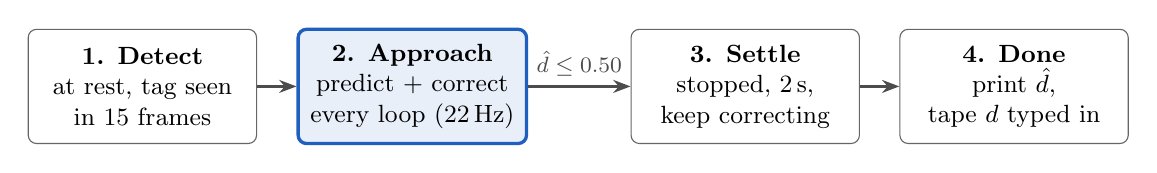
\begin{tikzpicture}[
  box/.style={draw=black!60,rounded corners=3pt,minimum width=2.9cm,minimum height=1.45cm,align=center,font=\small},
  key/.style={box,draw=acc,line width=1.2pt,fill=acc!10},
  arr/.style={-{Stealth[length=2.2mm]},black!70,thick}]
\node[box] (d) at (0,0) {\textbf{1. Detect}\\at rest, tag seen\\in 15 frames};
\node[key,right=0.5cm of d] (a) {\textbf{2. Approach}\\predict + correct\\every loop (22\,Hz)};
\node[box,right=1.3cm of a] (s) {\textbf{3. Settle}\\stopped, 2\,s,\\keep correcting};
\node[box,right=0.5cm of s] (o) {\textbf{4. Done}\\print $\hat d$,\\tape $d$ typed in};
\draw[arr] (d) -- (a); \draw[arr] (a) -- node[above,font=\footnotesize]{$\hat d\le0.50$} (s); \draw[arr] (s) -- (o);
\end{tikzpicture}
\caption{One trial. The blue step is where prediction and correction run; the robot stops on its own estimate, not on the tape.}
\end{figure}

\begin{figure}[H]\centering
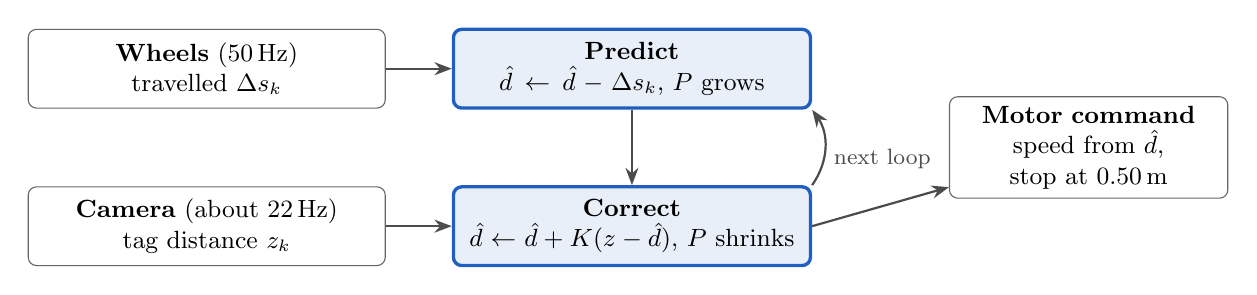
\begin{tikzpicture}[
  b/.style={draw=black!60,rounded corners=3pt,text width=4.3cm,minimum height=1.0cm,align=center,font=\small},
  k/.style={b,draw=acc,line width=1.2pt,fill=acc!10},
  arr/.style={-{Stealth[length=2.2mm]},black!70,thick}]
\node[b] (w) at (0,0) {\textbf{Wheels} (50\,Hz)\\travelled $\Delta s_k$};
\node[k] (p) at (5.4,0) {\textbf{Predict}\\$\hat d \leftarrow \hat d-\Delta s_k$,\ $P$ grows};
\node[b] (c) at (0,-2.0) {\textbf{Camera} (about 22\,Hz)\\tag distance $z_k$};
\node[k] (u) at (5.4,-2.0) {\textbf{Correct}\\$\hat d \leftarrow \hat d+K(z-\hat d)$,\ $P$ shrinks};
\node[b,text width=3.3cm] (m) at (11.2,-1.0) {\textbf{Motor command}\\speed from $\hat d$, stop at 0.50\,m};
\draw[arr] (w) -- (p); \draw[arr] (c) -- (u); \draw[arr] (p) -- (u); \draw[arr] (u.east) -- (m); \draw[arr] (u.north east) to[bend right=35] node[right,font=\footnotesize,pos=0.35]{next loop} (p.south east);
\end{tikzpicture}
\caption{The estimation loop. Odometry moves the estimate every loop; the camera pulls it back to the truth.}
\end{figure}

% ---------------------------------------------------------------------------------------
\section{Point 1: Video}
\begin{itemize}
  \item \textbf{Phone video of the trials:} \phonevideo
  \item \textbf{On-board camera view, saved by the program for every trial} (live estimate drawn on the image), on GitHub:
  \href{\gh/logs/trials/trial_08.mp4}{trial 8} (error $+4.5$\,mm),
  \href{\gh/logs/trials/trial_10.mp4}{trial 10} ($+4.9$\,mm),
  \href{\gh/logs/trials/trial_03.mp4}{trial 3} ($+43.9$\,mm, the largest); all ten are in \texttt{Assignment 3/logs/trials/}.
\end{itemize}
What to see: the robot waits until the tag is seen, accelerates to 0.20\,m/s, slows down as $\hat d$ approaches 0.50\,m, and stops; it rolls on for only 0.7--1.3\,cm after the stop command.

% ---------------------------------------------------------------------------------------
\section{Point 2: Where it is in the GitHub code}
Everything runs in one Python program on the laptop (no ROS), through the DJI RoboMaster SDK over a USB cable.
\begin{center}\small
\begin{tabularx}{\linewidth}{@{}>{\raggedright\arraybackslash}p{6.3cm}X@{}}
\toprule
\textbf{File, line} & \textbf{What happens there}\\
\midrule
\code{rm_odom_tag/kf.py}{L22}, line 22 & \texttt{predict}: subtract the travelled distance, grow the uncertainty (Eq.~\ref{eq:pred}).\\
\code{rm_odom_tag/kf.py}{L27}, line 27 & \texttt{correct}: gate check, gain $K$, update (Eqs.~\ref{eq:gate}--\ref{eq:upd}).\\
\code{rm_odom_tag/kf.py}{L69}, line 69 & \texttt{latency\_compensate}: move a late camera frame to the present (Eq.~\ref{eq:lat}).\\
\code{rm_odom_tag/tag.py}{L34}, line 34 & \texttt{plane\_distance}: perpendicular distance to the tag plane from the tag pose.\\
\code{rm_odom_tag/tag.py}{L106}, line 106 & \texttt{CameraModel.distance}: calibration $a z+b$ (Eq.~\ref{eq:cal}).\\
\code{rm_odom_tag/robot_io.py}{L63}, line 63 & subscribe to the chassis position at 50\,Hz (wheel odometry).\\
\code{rm_odom_tag/robot_io.py}{L98}, line 98 & \texttt{drive\_speed}: the command sent to the robot (0.5\,s watchdog).\\
\code{rm_odom_tag/trial.py}{L70}, lines 70--118 & one trial: predict (70), correct (83), stop rule (101), drive (118).\\
\code{rm_odom_tag/control.py}{L14}, line 14 & speed law and stop rule (Eqs.~\ref{eq:v}, \ref{eq:stop}).\\
\code{run_trials.py}{}, \code{scripts/analyze.py}{} & session driver (check, calib, warm-up, trials) and the error statistics.\\
\bottomrule
\end{tabularx}
\end{center}

% ---------------------------------------------------------------------------------------
\section{Point 3: Theory and formulas}
\subsection*{Prediction from odometry (motion model)}
The wheels report the travelled distance $s_k$. Between two loops the robot moves $\Delta s_k=s_k-s_{k-1}$ closer to the tag:
\begin{equation}\label{eq:pred}
\hat d_{k|k-1}=\hat d_{k-1}-\Delta s_k,\qquad P_{k|k-1}=P_{k-1}+(\alpha\,\Delta s_k)^2+(\sigma_v\,\Delta t)^2,
\end{equation}
with $\alpha=0.03$ (3\,\% wheel-slip uncertainty) and $\sigma_v=0.005$\,m/s. It starts at $\hat d_0=d_0=1.50$\,m with $\sigma_0=1$\,cm. Without correction this is just $d_0-s_k$: every slip and every placement error stays in the answer.

\subsection*{The camera measurement (sensor model)}
OpenCV finds the four corners of Tag~3 (tag36h11, 15\,cm); \texttt{solvePnP} gives the tag position $\mathbf t$ and its face direction $\mathbf n$. The distance to the tag \emph{plane} is $z_{plane}=|\mathbf n^\top\mathbf t|$. A linear calibration, fitted at rest against the tape at 12 positions, maps it to the reference point:
\begin{equation}\label{eq:cal}
z=a\,z_{plane}+b,\qquad a=0.9724,\ b=-0.0389\text{ m},\qquad \sigma_z=9.4\text{ mm}+4.4\text{ mm/m}^2\,z^2 .
\end{equation}
A frame is $L=0.015$\,s old when it arrives (measured in 2 warm-up runs), so it is shifted by the distance driven since then:
\begin{equation}\label{eq:lat}
z_k=z-\big[s(t_k)-s(t_k-L)\big].
\end{equation}

\subsection*{Correction (Kalman update)}
\begin{equation}\label{eq:gate}
y_k=z_k-\hat d_{k|k-1},\qquad S_k=P_{k|k-1}+R_k,\qquad \text{reject if } |y_k|>3\sqrt{S_k},
\end{equation}
\begin{equation}\label{eq:upd}
K_k=\frac{P_{k|k-1}}{S_k},\qquad \hat d_k=\hat d_{k|k-1}+K_k\,y_k,\qquad P_k=(1-K_k)\,P_{k|k-1},
\end{equation}
with $R_k=\sigma_z^2+(0.03\,v)^2$ (camera noise plus the latency uncertainty while moving). When odometry is uncertain ($P$ large) $K\to1$ and the camera dominates; when the camera is noisy ($R$ large) $K\to0$ and odometry dominates. The 3$\sigma$ gate rejected 2 of 2323 camera frames.

\subsection*{Motion and stop rule}
\begin{gather}
v_k=\mathrm{clip}\big(0.8\,(\hat d_k-d_{stop}),\ 0.04,\ 0.20\big)\ \text{m/s},\qquad |v_k-v_{k-1}|\le 0.25\,\Delta t,\label{eq:v}\\
\omega_k=\mathrm{clip}(1.2\,\beta_k,\ \pm15^\circ\!/\text{s}),\nonumber
\end{gather}
\begin{equation}\label{eq:stop}
\text{stop when}\quad \hat d_k-d_{stop}\le v_k\cdot 0.10\text{ s}.
\end{equation}
$\beta_k$ is the bearing of the tag in the image; it keeps the robot pointed straight at the tag.

% ---------------------------------------------------------------------------------------
\section{Point 4: What was used}
\begin{center}\small
\begin{tabularx}{\linewidth}{@{}>{\bfseries}p{3.6cm}X@{}}
\toprule
\textnormal{\textbf{Item}} & \textbf{Details}\\
\midrule
Robot & DJI RoboMaster EP Core, USB cable (RNDIS, robot at 192.168.42.2), camera 1280$\times$720.\\
Laptop software & Ubuntu 24.04, Python 3.12, \texttt{robomaster} SDK, OpenCV (ArUco/AprilTag detector), NumPy, SciPy, Matplotlib.\\
Tag & AprilTag 36h11 ID 3, black square 15\,cm, printed on A4, upright on a stand.\\
Measurement & Steel tape, 1\,mm marks, from the tag face to the front armour, on the centre line.\\
Place & Dorm room, carpet floor, indoor ceiling lights.\\
Experiment & Start 1.50\,m, stop 0.50\,m, 10 measured trials (plus 2 warm-up runs, not counted).\\
\bottomrule
\end{tabularx}
\end{center}

% ---------------------------------------------------------------------------------------
\section{Point 5: Error calculation}
After each trial the robot is left where it stopped and the tape distance $d_i$ is measured. The error of trial $i$ is
\begin{equation}
e_i=\hat d_i-d_i\qquad(\text{positive}=\text{the robot thought it was further away than it was}).
\end{equation}
Over the $n=10$ trials:
\begin{equation}
\bar e=\frac1n\sum e_i,\qquad \text{MAE}=\frac1n\sum|e_i|,\qquad s=\sqrt{\tfrac{1}{n-1}\sum(e_i-\bar e)^2},\qquad \text{range}=\max e_i-\min e_i .
\end{equation}
The same $e_i$ is computed for odometry alone ($d_0-s$) and the camera alone (camera at rest), to show what each part contributes.

\begin{center}\small
\begin{tabular}{@{}lrrr@{}}\toprule
 & \textbf{Fused KF} & Odometry only & Camera only\\\midrule
MAE (mm) & \textbf{21.0} & 31.3 & 22.3\\
Range of errors (mm) & \textbf{39.4} & 101.2 & 41.0\\
Smallest / largest error (mm) & +4.5 / +43.9 & $-33.3$ / +68.0 & +4.9 / +45.9\\
\bottomrule\end{tabular}
\end{center}

% ---------------------------------------------------------------------------------------
\section{Point 6: Error correction}
Odometry alone has two problems: it assumes the robot started exactly at 1.50\,m, and wheel slip adds up during the drive. The camera fixes both. Figure~\ref{fig:all}(b) shows, for every trial, how far the camera moved the estimate away from the odometry-only value. At the end of the trials this correction was between $-37.4$ and $+46.3$\,mm: in trial 6 the robot was placed about 4\,cm behind the mark, and the camera found and removed that.
\begin{itemize}
  \item Result: the fused MAE is \textbf{33\,\% lower} than odometry alone (21.0 vs 31.3\,mm), and the spread of the errors is \textbf{2.6 times smaller} (range 39.4 vs 101.2\,mm).
  \item What remains is one common offset: all ten errors are positive (bias +21.0\,mm). The fused errors follow the camera errors within 3\,mm, so the remaining offset comes from the camera calibration (no calibration point below 0.75\,m), not from the filter. Adding calibration points at 0.50 and 1.00\,m is the next fix.
\end{itemize}

% ---------------------------------------------------------------------------------------
\section{Point 7: Graphs}
\begin{figure}[H]\centering
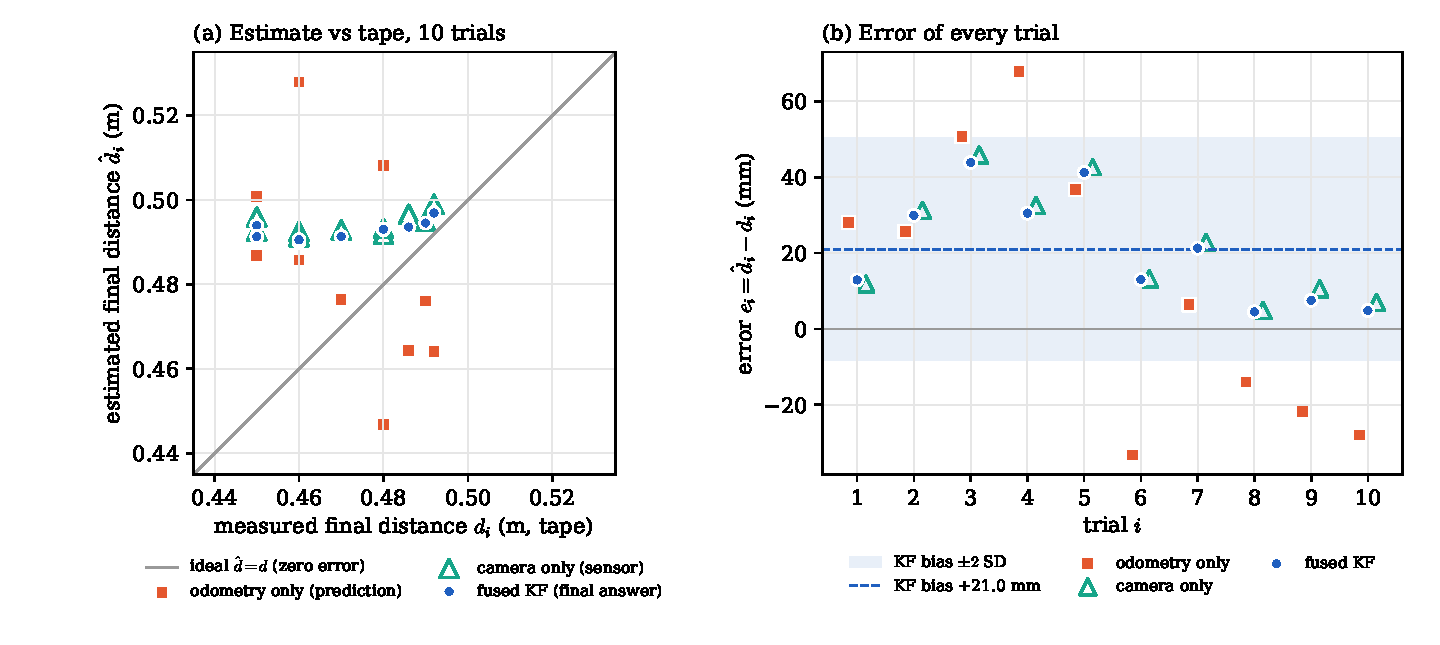
\includegraphics[width=\linewidth]{fig_final.pdf}
\caption{Final results, scatter plots. (a) Estimate against tape for all 10 trials: the closer to the diagonal, the better. The fused points (blue) and camera points (green) form a tight row; odometry (orange) is scattered. (b) Error of every trial, with the fused bias and its $\pm2$\,SD band.}
\end{figure}
\begin{figure}[H]\centering
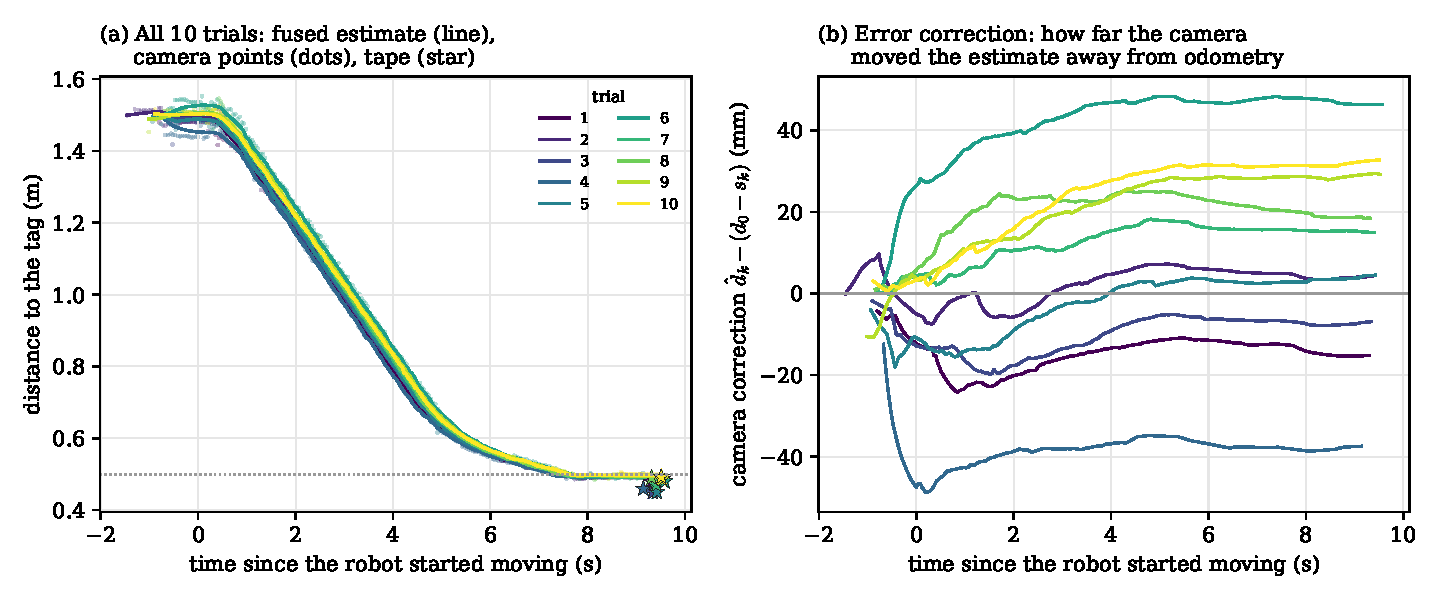
\includegraphics[width=\linewidth]{fig_all_trials.pdf}
\caption{All 10 trials in one graph. (a) Fused distance estimate of each trial over time, with the camera measurements as dots and the tape measurement as a star at the end. (b) The correction applied by the camera in each trial.}\label{fig:all}
\end{figure}

% ---------------------------------------------------------------------------------------
\section{Point 8: Statistical analysis}
\begin{center}\small
\begin{tabular}{@{}lrrr@{}}\toprule
Statistic (mm unless stated) & Fused KF & Odometry only & Camera only\\\midrule
Trials $n$ & 10 & 10 & 10\\
Mean error (bias) $\bar e$ & +21.0 & +11.9 & +22.3\\
Standard deviation $s$ & 14.7 & 35.2 & 15.0\\
Mean absolute error (MAE) & 21.0 & 31.3 & 22.3\\
Root mean square error (RMSE) & 25.2 & 35.5 & 26.4\\
Median error & +17.2 & +16.1 & +18.0\\
Minimum error & +4.5 & -33.3 & +4.9\\
Maximum error & +43.9 & +68.0 & +45.9\\
Range of errors $e_{max}-e_{min}$ & 39.4 & 101.2 & 41.0\\
Largest $|e_i|$ & 43.9 & 68.0 & 45.9\\
95\,\% CI of the bias & [+10.5, +31.5] & [-13.3, +37.1] & [+11.5, +33.0]\\
$t$-test $H_0{:}\ \bar e=0$, $p$ & 0.001 & 0.314 & 0.001\\
Shapiro--Wilk normality, $p$ & 0.230 & 0.536 & 0.235\\
\midrule
Wilcoxon $|e_{KF}|$ vs $|e|$ of this method, $p$ & -- & 0.064 & 0.010\\
\bottomrule\end{tabular}

\end{center}
\begin{figure}[H]\centering
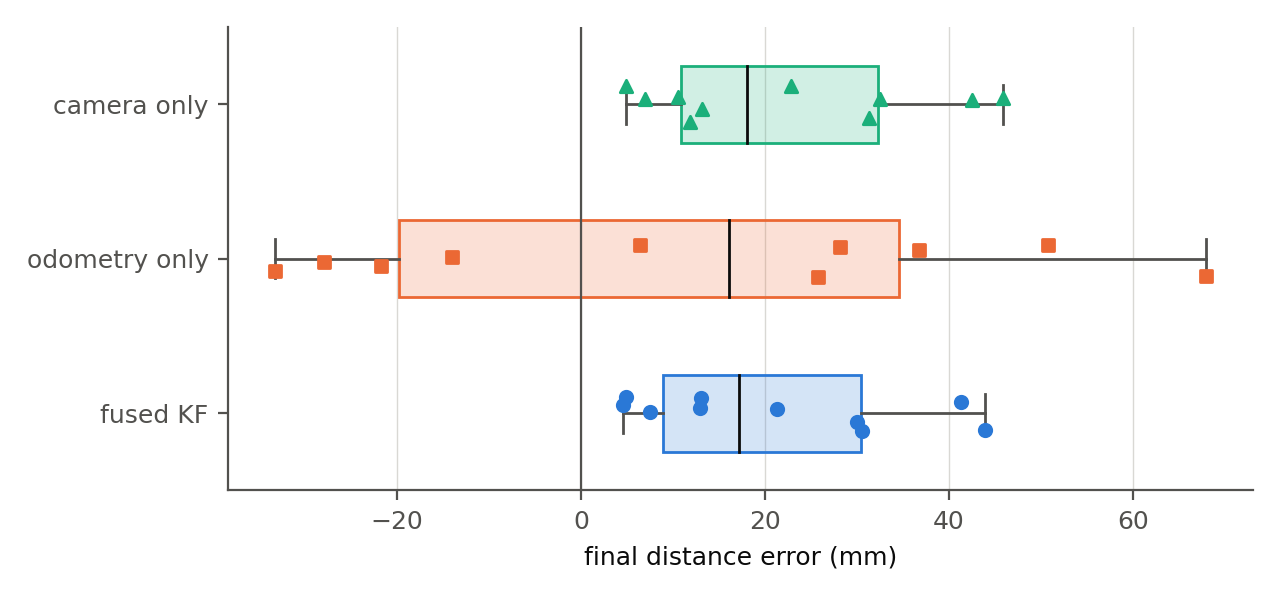
\includegraphics[width=0.78\linewidth]{../figures/fig_error_box.png}
\caption{Distribution of the final errors (box: middle 50\,\%, line: median, points: the 10 trials).}
\end{figure}
\begin{itemize}
  \item \textbf{Is there a systematic error?} Yes for the fused estimate: bias +21.0\,mm, 95\,\% confidence interval [+10.5, +31.5]\,mm, $t$-test $p=0.001$. The interval does not include zero.
  \item \textbf{Is it normal?} Shapiro--Wilk $p=0.23$: no evidence against a normal distribution, so the $t$-interval is valid.
  \item \textbf{Is fused better than odometry?} MAE 21.0 vs 31.3\,mm and SD 14.7 vs 35.2\,mm. The paired Wilcoxon test gives $p=0.064$: a clear improvement in spread, but with only 10 trials the MAE difference is just above the 5\,\% level.
  \item \textbf{Is fused better than camera only?} Slightly (MAE 21.0 vs 22.3\,mm, Wilcoxon $p=0.010$); during motion the filter also gives a smooth estimate that the camera alone cannot.
  \item \textbf{Repeatability:} the robot's real stopping distance had SD 16.0\,mm; the last three trials, after the tag stand was fixed in place, were within 8\,mm.
\end{itemize}

\end{document}
